\documentclass[3p, authoryear]{elsarticle} %review=doublespace preprint=single 5p=2 column
%%% Begin My package additions %%%%%%%%%%%%%%%%%%%
\usepackage[hyphens]{url}

  \journal{Submitted to Journal} % Sets Journal name


\usepackage{lineno} % add
\providecommand{\tightlist}{%
  \setlength{\itemsep}{0pt}\setlength{\parskip}{0pt}}

\usepackage{graphicx}
%%%%%%%%%%%%%%%% end my additions to header

\usepackage[T1]{fontenc}
\usepackage{lmodern}
\usepackage{amssymb,amsmath}
\usepackage{ifxetex,ifluatex}
\usepackage{fixltx2e} % provides \textsubscript
% use upquote if available, for straight quotes in verbatim environments
\IfFileExists{upquote.sty}{\usepackage{upquote}}{}
\ifnum 0\ifxetex 1\fi\ifluatex 1\fi=0 % if pdftex
  \usepackage[utf8]{inputenc}
\else % if luatex or xelatex
  \usepackage{fontspec}
  \ifxetex
    \usepackage{xltxtra,xunicode}
  \fi
  \defaultfontfeatures{Mapping=tex-text,Scale=MatchLowercase}
  \newcommand{\euro}{€}
\fi
% use microtype if available
\IfFileExists{microtype.sty}{\usepackage{microtype}}{}
\usepackage{natbib}
\bibliographystyle{apalike}
\usepackage{longtable,booktabs,array}
\usepackage{calc} % for calculating minipage widths
% Correct order of tables after \paragraph or \subparagraph
\usepackage{etoolbox}
\makeatletter
\patchcmd\longtable{\par}{\if@noskipsec\mbox{}\fi\par}{}{}
\makeatother
% Allow footnotes in longtable head/foot
\IfFileExists{footnotehyper.sty}{\usepackage{footnotehyper}}{\usepackage{footnote}}
\makesavenoteenv{longtable}
\usepackage{graphicx}
\ifxetex
  \usepackage[setpagesize=false, % page size defined by xetex
              unicode=false, % unicode breaks when used with xetex
              xetex]{hyperref}
\else
  \usepackage[unicode=true]{hyperref}
\fi
\hypersetup{breaklinks=true,
            bookmarks=true,
            pdfauthor={},
            pdftitle={ATSPM Data Analysis},
            colorlinks=false,
            urlcolor=blue,
            linkcolor=magenta,
            pdfborder={0 0 0}}
\urlstyle{same}  % don't use monospace font for urls

\setcounter{secnumdepth}{5}
% Pandoc toggle for numbering sections (defaults to be off)

% Pandoc citation processing

% Pandoc header
\usepackage{booktabs}
\usepackage{booktabs}
\usepackage{longtable}
\usepackage{array}
\usepackage{multirow}
\usepackage{wrapfig}
\usepackage{float}
\usepackage{colortbl}
\usepackage{pdflscape}
\usepackage{tabu}
\usepackage{threeparttable}
\usepackage{threeparttablex}
\usepackage[normalem]{ulem}
\usepackage{makecell}
\usepackage{xcolor}
\usepackage{siunitx}
\newcolumntype{d}{S[input-symbols = ()]}



\begin{document}
\begin{frontmatter}

  \title{ATSPM Data Analysis}
    \author[Brigham Young University]{Matthew Davis\corref{1}}
   \ead{mabosdavis@gmail.com} 
    \author[Brigham Young University]{Gregory Macfarlane\corref{2}}
   \ead{gregmacfarlane@byu.edu} 
      \address[Brigham Young University]{Civil and Environmental Engineering Department, 430 Engineering Building, Provo, Utah 84602}
      \cortext[1]{Corresponding Author}
    \cortext[2]{Present affiliation: some nice job}
  
  \begin{abstract}
  This is where the abstract should go.
  \end{abstract}
   \begin{keyword} Accessibility Passive Data Location Choice\end{keyword}
 \end{frontmatter}

\hypertarget{intro}{%
\section{Question}\label{intro}}

Since December 2019, the COVID-19 pandemic has affected life around the world in an unprecedented manner. Mask mandates, social distancing, and stay-at-home orders have changed the way society lives, works, and interacts. With these safety precautions have come less interaction, traveling, and driving on roads and highways. Recent research has confirmed that the COVID-19 pandemic has led to a decrease in traffic volumes across the United States and the world.

Although this is a recent event, the topic has already been researched in many states and countries \citep{Lee2020, Lee2021, Muley2021}, but has not been specifically looked at for Utah and Salt Lake Counties in Utah, USA. These counties also contain signal specific traffic volume detectors, which provide a detailed insight into the variation of the effect of COVID-19 on traffic volumes in different locations. The research question therefore is:

\begin{itemize}
\tightlist
\item
  What was the effect of COVID-19 on traffic volumes in Utah and Salt Lake Counties?
\end{itemize}

\hypertarget{methods}{%
\section{Methods}\label{methods}}

UDOT provided volume data for many signals, but for the purposes of this research, significantly fewer signals were actually analyzed. Data was collected from traffic volume detectors in Provo, Orem, and Cottonwood Heights, Utah and then processed through UDOT's Automated Traffic Signal Performance Measures (ATSPM) system. Data was provided for downtown Provo, Orem State Street, University Avenue, Orem 800 N, and Fort Union Boulevard in Cottonwood Heights for the years 2017-2020, but many of the data were plagued by detector issues. Common issues ranged from shifting of the data up or down considerably and then shifting back after a period of time, missing data, or lack of data in general. Only four signals from Fort Union Blvd and three signals from Orem 800 N were ultimately deemed as complete and consistent enough to be used in the analysis.

A general linear regression and four fixed effect models were created to evaluate the effect of COVID-19 on volume in the aforementioned corridors. Fixed effects models were created for day of the week, month, whether or not it was during the COVID-19 pandemic, and individual signals. To divide the Pre COVID-19 time period from the COVID-19 time period, a separation date was chosen. In Utah, on March 12, 2020, Governor Cox announced that gatherings over 100 people should be canceled, as well as many of the universities in the state making the formal announcement that they would transition to online school for the remainder of the semester. These announcements were one of the first events of the pandemic that directly affected the lives of the public in Utah, hence it being chosen as the separation date.

\begin{figure}
\centering
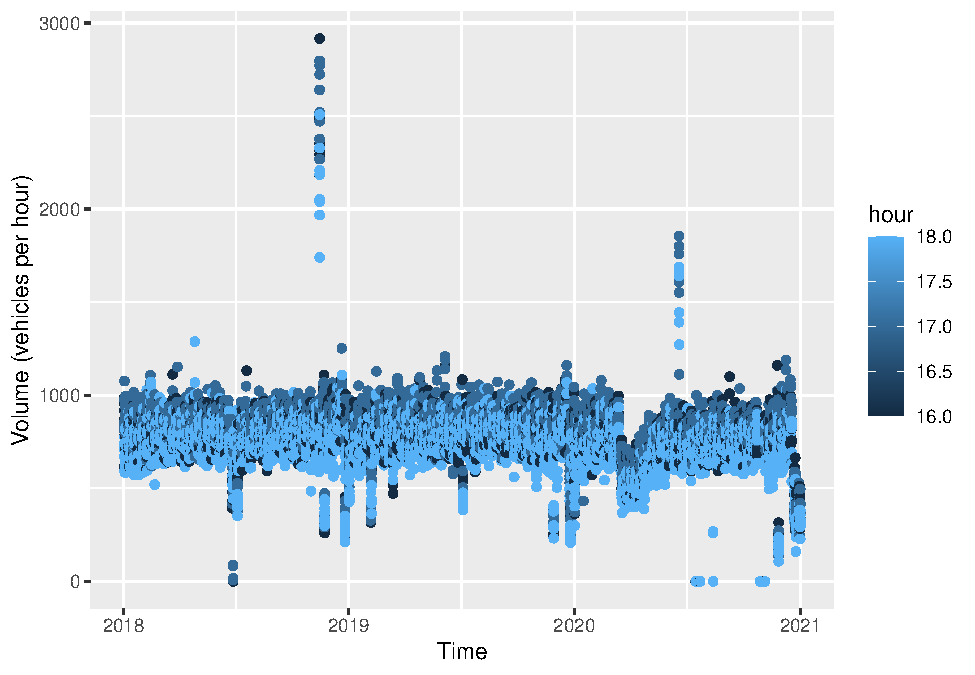
\includegraphics{ATSPM_data_analysis_files/figure-latex/datasummary-1.pdf}
\caption{\label{fig:datasummary}Traffic volumes at State St and 800 N in Orem, UT before and during the COVID-19 pandemic.}
\end{figure}

Variation in traffic volumes are dependent on multiple factors such as season, time of day, and day of the week. These three factors were controlled for and were limited to focus the analysis. For days of the week, only Tuesday, Wednesday and Thursday were analyzed. The density of vehicles was greatest during the hours of 7AM to 9AM and 4PM to 6PM, or the ``AM Peak'' and ``PM Peak'' respectively, but only the ``PM Peak'' data were used in the analysis. Other potential factors include weather and road conditions, sporting events and major holidays. Theses were not accounted for in the analysis.

\hypertarget{findings}{%
\section{Findings}\label{findings}}

During the analysis, several variables were found to have a statistically significant effect on traffic. Month of the year, the time period of the COVID-19 pandemic, and difference in traffic signals were all found to have a significant effect on vehicles per hour of phases 2 and 6 of the signals specified in the methods section. This is seen in Table \ref{tab:general}.

Each individual factor was given a fixed effects model to further investigate where significant factors occurred. Table \ref{tab:FEmonth} shows that with January as the reference, each month, except for May, was statistically significant. Standard errors were similar across the year, with beta intercepts vary widely. The effect of day of the week though was the complete opposite. Table \ref{tab:FEday} shows that day of the week had little to no affect on variations in hourly volume. Difference in whether or not a date was occuring after March 12, 2021, which was assumed to be the start of the COVID-19 pandemic shutdown in Utah, was shown to be significant in Table \ref{tab:FECOVID}. Individual signals were also shown to be significant in Table \ref{tab:FESignal}.

Like with any research, there were significant limitations to the data and analyses. Through the data cleaning process, it became very clear that many of the data provided were not complete or contained detector errors, leaving most of the data unusable. From 52 signals originally with data, only 7 were used in this analysis. Even with the most accurate data available, further detector error or unknown errors could be present. Other factors such as weather, holidays and major events, school openings, weather, and road conditions were not controlled for.

While not perfect, this analysis provides the conclusion that despite seasonal and signal specific variation, hourly volumes were significantly affected by the COVID-19 pandemic.

Note: The Methods section still needs to be updated to reflect the changes in methodology made in the last few days.

Base controls for Signals, COVID is base, but also controlling for COVID. Controls is Base controlling for everything, including day of week and month. R-squared value goes up, beta for COVID becomes more pronounced, quantify how much of an effect COVID had.

\begin{table}
\centering
\begin{tabular}[t]{lccc}
\toprule
  & Base & COVID & Controls\\
\midrule
Intercept & \num{597.659}*** & \num{613.964}*** & \num{583.915}***\\
\addlinespace[0.3em]
\multicolumn{4}{l}{\textbf{Signal}}\\
\hspace{1em}4090 & \num{-144.368}*** & \num{-144.014}*** & \num{-143.891}***\\
\hspace{1em}4704 & \num{-256.367}*** & \num{-256.367}*** & \num{-256.367}***\\
\hspace{1em}4705 & \num{-297.147}*** & \num{-297.147}*** & \num{-297.147}***\\
\hspace{1em}6303 & \num{521.797}*** & \num{521.797}*** & \num{521.797}***\\
\hspace{1em}6304 & \num{587.444}*** & \num{587.444}*** & \num{587.444}***\\
\hspace{1em}6307 & \num{361.787}*** & \num{374.462}*** & \num{369.262}***\\
\addlinespace[0.3em]
\multicolumn{4}{l}{\textbf{COVID-19}}\\
\hspace{1em}\textcolor{red}{COVID} & \textcolor{red}{} & \textcolor{red}{\num{-60.470}***} & \textcolor{red}{\num{-64.316}***}\\
\addlinespace[0.3em]
\multicolumn{4}{l}{\textbf{Month}}\\
\hspace{1em}February &  &  & \num{40.496}***\\
\hspace{1em}March &  &  & \num{-4.807}\\
\hspace{1em}April &  &  & \num{-49.007}***\\
\hspace{1em}May &  &  & \num{18.477}***\\
\hspace{1em}June &  &  & \num{68.951}***\\
\hspace{1em}July &  &  & \num{66.158}***\\
\hspace{1em}August &  &  & \num{81.054}***\\
\hspace{1em}September &  &  & \num{67.783}***\\
\hspace{1em}October &  &  & \num{35.628}***\\
\hspace{1em}November &  &  & \num{33.557}***\\
\hspace{1em}December &  &  & \num{18.169}***\\
\addlinespace[0.3em]
\multicolumn{4}{l}{\textbf{Day}}\\
\hspace{1em}Wednesday &  &  & \num{-2.018}\\
\hspace{1em}Thursday &  &  & \num{2.368}\\
\midrule
Num.Obs. & \num{147888} & \num{147888} & \num{147888}\\
R2 & \num{0.515} & \num{0.518} & \num{0.524}\\
F & \num{26192.568} & \num{22729.455} & \num{8127.656}\\
\bottomrule
\end{tabular}
\end{table}

\bibliography{book.bib}


\end{document}
